% create the illustration of vector transformation
% between full state space and slice.
% use package tikz
% By Xiong
% 
% use the following command to generate the pdf
% pdflatex --jobname=jacobian-f1 jacobian.tex 

\documentclass{article}
\usepackage{graphicx}
\usepackage{tikz}

\pgfrealjobname{jacobian}

\begin{document}

\beginpgfgraphicnamed{jacobian-f1}
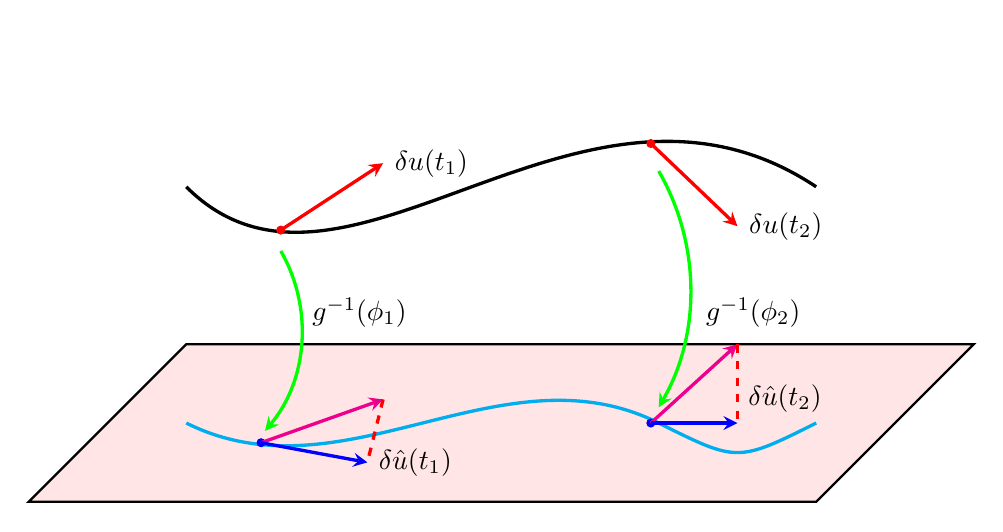
\begin{tikzpicture}

  % coordinates for the rectangle
  \coordinate (A) at (0, 0);
  \coordinate (B) at (10, 0);
  \coordinate (C) at (12, 2);
  \coordinate (D) at (2, 2);

  % coordinate for the curve in the full state space
  \coordinate (sp1) at (2, 4);
  \coordinate (sp2) at (4, 2);
  \coordinate (sp3) at (7, 6);
  \coordinate (sp4) at (10, 4);

  % coordinate for the curve in the slice
  \coordinate (rsp1) at (2, 1);
  \coordinate (rsp2) at (4, 0);
  \coordinate (rsp3) at (6, 2);
  \coordinate (rsp4) at (8, 1);
  \coordinate (rsp5) at (9, 0.5);
  \coordinate (rsp6) at (10, 1);

  % draw the slice 
  \draw[thick, color=black, fill=red!10] (A) -- (B) -- (C) -- (D) -- cycle;
  
  % draw the curve in the full state space (a Bezier cure)
  \draw[very thick, black] 
  (sp1) .. controls (sp2) and (sp3) .. (sp4) ;

  % draw the curve in the slice (a Bezier cure)
  \draw[very thick, cyan]
  (rsp1) .. controls (rsp2) and (rsp3) .. (rsp4) ;
  \draw[very thick, cyan]
  (rsp4) .. controls (rsp5) .. (rsp6) ;

  % draw arrows 
  \draw[<-, >=stealth, color=green, very thick] (3, 0.9) arc(320:390:2);
  \draw[<-, >=stealth, color=green, very thick] (8, 1.2) arc(330:390:3);
  \node at (4.2, 2.4) {$g^{-1}(\phi_1)$} ;
  \node at (9.2, 2.4) {$g^{-1}(\phi_2)$} ;

  % draw vectors
  % delta x(t1)
  \coordinate  (t1) at (3.2, 3.45);
  \filldraw[color=red] (t1) circle(0.05);
  \draw[->, >=stealth, color=red, very thick] (t1) -- (4.5, 4.3) 
  node[color=black, right=0.3] {$\delta u(t_1)$};

  % delta x(t2)
  \coordinate  (t2) at (7.9, 4.55);
  \filldraw[color=red] (t2) circle(0.05);
  \draw[->, >=stealth, color=red, very thick] (t2) -- (9, 3.5) 
  node[color=black, right=0.3] {$\delta u(t_2)$};

  % delta \hat{x}(t1)
  \coordinate  (rt1a) at (2.95, 0.75);
  \coordinate  (rt1b) at (4.5, 1.3);
  \coordinate  (rt1c) at (4.3, 0.5) ;
  \filldraw[color=blue] (rt1a) circle(0.05);
  \draw[->, >=stealth, color=magenta, very thick] (rt1a) -- (rt1b);
  \draw[dashed, color=red, very thick] (rt1b)  -- (rt1c);
  \draw[->, >=stealth, color=blue, very thick] (rt1a) -- (rt1c) 
  node[color=black, right=0.2] {$\delta \hat{u}(t_1)$};

  % delta \hat{x}(t2)
  \coordinate  (rt1a) at (7.9, 1);
  \coordinate  (rt1b) at (9, 2);
  \coordinate  (rt1c) at (9, 1) ;
  \filldraw[color=blue] (rt1a) circle(0.05);
  \draw[->, >=stealth, color=magenta, very thick] (rt1a) -- (rt1b);
  \draw[dashed, color=red, very thick] (rt1b)  -- (rt1c);
  \draw[->, >=stealth, color=blue, very thick] (rt1a) -- (rt1c) 
  node[color=black, above right =0.05] {$\delta \hat{u}(t_2)$};

\end{tikzpicture}
\endpgfgraphicnamed

\end{document}